% !Mode:: "TeX:UTF-8"
%!TEX program  = xelatex

\documentclass{cumcmthesis}
\usepackage{graphicx}
\usepackage{float}
\usepackage{subfig}
\usepackage{footnote}
% \documentclass[withoutpreface,bwprint]{cumcmthesis} %去掉封面与编号页

\usepackage{url}
\title{繁花曲线的分析与绘制}
\tihao{A}
\baominghao{114514}
\schoolname{天元公学}
\membera{陈铭硕}
\memberb{唐铭泽}
\memberc{尹贝尔}
\supervisor{老师}
\date{\today}
\usepackage{footnote}

\usepackage{graphicx}
\usepackage{float}
\usepackage{subfig}

\begin{document}

\maketitle

\begin{abstract}

\keywords{疫情防控\quad  图论\quad   网络流\quad  最短路}
\end{abstract}

%目录
\tableofcontents

\newpage
\section{问题重述}

\subsection{问题的提出}

\section{问题分析}

\subsection{总体分析}

一个居民小区通常由一些单元与道路组成。每个单元都有一定数量的人居住,每条道路都有一定的长度。此外,我们可以把道路的交叉点等看作没有人居住的单元。核酸检测点可
以设在单元里,也可以设在道路上。于是我们可以把居民小区抽象为一张无向图,以单元为点,点权为居住人数,边权为边的长度,把核酸检测点的规划转化成图论问题进行求解。

\subsection{问题一分析}

定义图上两点的花费为两点的最短路径长度乘上起始点的点权。

建立核酸检测点位置要使居民总体方便,那么建立核酸检测点的位置有两种选择:一种是使得居民到达核酸检测点的总花费最短,另一种是使得到达核酸检测点的最大的花费最
小;并且需要考虑建立的位置是否会给居民的正常生活造成影响。

\subsection{问题二分析}

\subsection{问题三分析}

\section{模型假设}

\section{符号说明}
\begin{center}
\begin{savenotes}
\begin{tabular}{cc}
\hline
\makebox[0.3\textwidth][c]{符号}	&  \makebox[0.4\textwidth][c]{意义} \\ \hline
$n$         & 图的点数 \\ \hline
$m$         & 图的边数 \\ \hline
$w_i$	    & 第 $i$ 个点的点权 \\ \hline
$e_i$	    & 第 $i$ 条边的边权 \\ \hline
$u_i$       & 第 $i$ 条边的起点 \\ \hline
$v_i$       & 第 $i$ 条边的终点 \\ \hline
$d_{i,j}$   & 第 $i$ 个点和第 $j$ 个点最短路径长度 \\ \hline
\end{tabular}
\end{savenotes}
\end{center}

\section{模型建立、求解与分析}

\subsection{问题一}

\subsubsection{选择一}

使得居民到达核酸检测点的总花费最短。

首先对于每一对 $(i,j)$ 求出 $d_{i,j}$,然后考虑核酸检测点的位置。如果核酸检测点在边 $(u_k,v_k)$ 上,且距 $u$ 点的距离为 $x(x\le e_k)$,
那么它距 $v_k$ 的距离为 $e_k-x$。



\subsubsection{选择二}

使得到达核酸检测点的最大的花费最小。

提出一个概念叫 \emph{图的绝对重心},定义为到所有点的花费距离的最大值最小的点,那我们的核酸检测点应建立在绝对重心上。

接下来考虑如何求解绝对重心。

假设图的绝对重心在边上,枚举每一条边 $(u_k,v_k)$,钦定图的绝对重心 $c$ 在这一条边上,假设其距 $u_k$ 的距离为 $x(x \le e_k)$,那么它距离 $v_k$ 的距离为 $e_k - x$。

如图绝对重心 $c$ 与一点 $i$ 的关系图:

\begin{figure}[H]
    \centering
    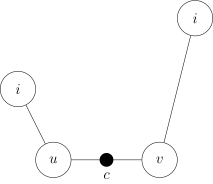
\includegraphics{images/mdst-graph.png}
    \caption{图的绝对中心与一点的位置关系\cite{oiwiki-dmst}}
    \label{fig:mdst-graph}
\end{figure}

那么 $d_{c,i} = \min\{w_i \times (d_{u_k, i} + x), w_i \times (d_{v_k,i} + e_k - x)\}$。

随着 $c$ 从 $u_k$ 到 $v_k$ 的移动 $d_{c,i}$ 的变化如图可以画到一个平面直角坐标系上:

\begin{figure}[H]
	\centering
	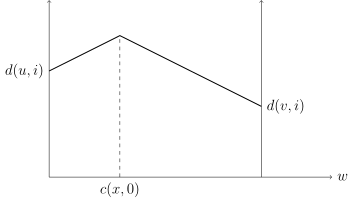
\includegraphics{images/mdst-plot1.png}
	\caption{图的绝对中心变化的影响\cite{oiwiki-dmst}}
	\label{fig:mdst-graph}
\end{figure}

然后显然可以发现图像会是两条斜率相同的一次函数所构成。

接下来将对于每一个点 $i$ 都画像这样的图像就可以得到:

\begin{figure}[H]
	\centering
	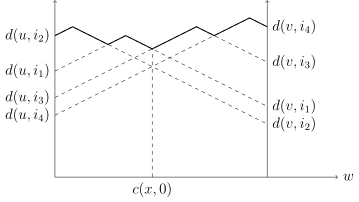
\includegraphics{images/mdst-plot2.png}
	\caption{图的绝对中心变化的影响\cite{oiwiki-dmst}}
	\label{fig:mdst-graph}
\end{figure}

这些折线交点中的最低点,横坐标就是图的绝对中心的位置。

对于绝对中心在一个点上,那么就枚举一下那个节点,再用与其距离最远的节点更新一下就行了。

对于每一条边,每一个点都这样做一下就可以了。

总结一下过程:

\begin{enumerate}
    \item 使用最短路算法求出 $d_{i,j}$;
    \item 对于绝对中心在点上更新答案;
    \item 对于绝对中心在边上,枚举每一条边更新答案;
\end{enumerate}

如果使用堆优化的 Dijkstra 求解最短路,时间复杂度为 $\Theta(n^2\log m + nm);若使用 使用 Floyd,时间复杂度为 $\Theta(n^3 + nm)$

\subsection{问题二}

我们发现

\section{模型评价}


\bibliographystyle{plain}
\bibliography{ref}
\newpage

%附录
\begin{appendices}


\section{问题一代码}

\begin{lstlisting}[language=cpp]
#include <iostream>
using namespace std;
typedef long long ll;
const ll INF = 1e18;

int N, M;
ll G[510][510], Dist[510][510], Rank[510][510], W[510];

void CenTer_Point(int &u, int &v, double &x) {
    for (int k = 1; k <= N; k++) {
        for (int i = 1; i <= N; i++) {
            for (int j = 1; j <= N; j++) {
                Dist[i][j] = min(Dist[i][j], Dist[i][k] + Dist[k][j]);
            }
        }
    }

    for (int i = 1; i <= N; i++) {
        for (int j = 1; j <= N; j++) Rank[i][j] = j;
        for (int j = 1; j <= N; j++) {
            for (int k = j + 1; k <= N; k++) {
                if (Dist[i][Rank[i][j]] > Dist[i][Rank[i][k]]) {
                    swap(Dist[i][Rank[i][j]], Dist[i][Rank[i][k]]);
                }
            }
        }
    }

    double Ans = 1e18;

    for (int i = 1; i <= N; i++) {
        for (int j = 1; j <= N; j++) {
            if (i == j || G[i][j] == INF) continue;
            int p = Rank[i][N];
            ll Temp = W[i] * Dist[i][p];
            if (Ans > Temp) {
                Ans = Temp;
                u = i;
                v = j;
                x = 0.00;
            }
            for (int k = N - 1; k >= 1; k--) {
                int t = Rank[i][k];
                if (Dist[j][t] > Dist[j][p]) {
                    Temp = W[i] * (Dist[i][t] + Dist[j][p] + G[i][j]);
                    if (Ans > Temp) {
                        Ans = Temp;
                        u = i;
                        v = j;
                        x = (Dist[j][p] + Dist[i][j] - Dist[i][t]) / 2.00;
                    }
                    p = t;
                }
            }
        }
    }

    return;
}
\end{lstlisting}

\end{appendices}

\end{document} 